\documentclass[10pt,a4paper]{article}
\usepackage[utf8]{inputenc}
\usepackage[english]{babel}
\usepackage[T1]{fontenc}
\usepackage{amsmath}
\usepackage{amsfonts}
\usepackage{amssymb}
\usepackage{makeidx}
\usepackage{graphicx}
\usepackage{fourier}
\usepackage{listings}
\usepackage{color}
\usepackage{hyperref}
\usepackage[left=2cm,right=2cm,top=2cm,bottom=2cm]{geometry}
\author{Johannes Scheller, Vincent Noculak, Lukas Powalla}
\title{Computational Physics - Project 3}

\lstset{language=C++,
	keywordstyle=\bfseries\color{blue},
	commentstyle=\itshape\color{red},
	stringstyle=\color{green},
	identifierstyle=\bfseries,
	frame=single}
\begin{document}

\maketitle
\newpage
\tableofcontents
\newpage

\begin{abstract}
		
	In this project, we look at different numerical integration methods applied on the problem of the correlation energy of two electrons in a helium atom. First we will study the Gauss-Legendre and Gauss-Laguerre quadrature and compare them to each other. Later we will evaluate the integral using a Monte Carlo calculation, which we will improve by using importance sampling. The usefulness of the different methods will be discussed.
	
\end{abstract}
	
\section{Introduction to Project 3}

We are looking at the six-dimensional integral, which is used to determine the ground state correlation energy between to electrons in a helium atom. This integral is given by: 
\begin{equation}
	I = \int\limits_{\mathbb{R}^6} d\mathbf{r_1} d\mathbf{r_2} e^{-4 (r_1+r_2)} \frac{1}{|\mathbf{r_1} - \mathbf{r_2}|} 
\end{equation}

Or in spherical coordinates:

\begin{align}
	\begin{split}
		I = \int_0^\infty \int_0^\infty  \int_0^{2 \pi} \int_0^{2 \pi}  \int_0^\pi \int_0^\pi dr_1 dr_2 d\theta_1 d\theta_2 d\phi_1 d\phi_2    r_1^2 r_2^2 sin(\theta_1) sin(\theta_2)\\ \cdot \frac{e^{-4(r_1+r_2)}} {\sqrt{r_1^2+r_2^2-r_1r_2(cos(\theta_1)cos(\theta_2)+sin(\theta_1)sin(\theta_2)cos(\phi_1-\phi_2))}}
	\end{split}
\end{align}

The analytical solution of this integral is $I = \frac{5 \pi^2}{16^2}$.

To solve this integral numerical. We will first apply the Gauss-Legendre quadrature for every variable in Cartesian coordinates. After that we use the Gauss-Laguerre quadrature in Spherical coordinates. Next we will study the solution for the Monte Carlo method. Where we first apply a brute force algorithm in Cartesian coordinates and then improve the algorithm with importance sampling, by eliminating the exponential term of the integral.

\section{Theory}
\subsection{Gauss-Legendre and Gauss-Laguerre quadrature}

In Gaussian quadrature we use the characteristics of orthogonal polynomials to numerically integrate a function. The Legendre polynomials which are of such kind are defined in the interval $[-1;1]$. Using mapping we can use the Gauss-Legendre quadrature for an integral with any integration limits $a, b \in \mathbb{R}$. In our case we can make the approximation $\int_{\infty}^{\infty} f(\mathbf{r_1},\mathbf{r_2}) \approx \int_{-a}^{a} f(\mathbf{r_1},\mathbf{r_2})$ in case "a" is high enough, because the value of our function decreases very quickly due to the exponential function. The value of the numerically calculated integral in six dimensions is given by:

\begin{align}
	I = \sum_{f,g,h,i,j,k = 1}^{n}\omega_f \cdot \omega_g \cdot \omega_h \cdot \omega_i \cdot \omega_j \cdot \omega_k \cdot f(x_{1,f} , x_{2,g} , y_{1,h} , y_{2,i} , z_{1,j} , z_{2,k})  
\end{align}

Where $f$ is the function we want to integrate, $x_i$ is a point where the Legendre polynomial of degree n is zero and $\omega_i$ can be seen a the weight of this point.

Gauss-Laguerre quadrature is especially good to numerically solve integrals of the form $\int_{0}^{\infty} e^{-\alpha x} f(x) dx$. As seen in (2), we have such an integral if we use Spherical coordinates. Hence we will integrate $r_1$ and $r_2$ in Spherical coordinates with Gauss-Laguerre, while we integrate $\theta_1$, $\theta_2$, $\phi_1$ and $\phi_2$ with Gauss-Legendre quadrature. The formula will have the same form as (3).

\subsection{Monte-Carlo-Method} 

In the Monte-Carlo integration we make use of the fact, that you can write an integral of a function as the expectation value of this function with the uniform distribution.

\begin{equation}
	I = \int_{a}^{b} f(x) dx = <f> \approx \frac{(b-a)}{n} \sum_{i=1}^{n} f(x_i)
\end{equation}

Hence in our case we can write our integral as:

\begin{equation}
	I = \frac{(2a)^6}{n} \sum_{i = 1}^n f(x_{1,i}, x_{2,i}, y_{1,i}, y_{2,i}, z_{1,i}, z_{2,i})
\end{equation}

Where the $x_i$'s, $y_i$'s and $z_i$'s are random generated numbers in the interval $[-a;a]$ ($a \in \mathbb{R}$) with an uniform distribution. If we choose "a" big enough this is a good approximation to the integration limits(which are infinite), because the value of our function decreases quickly. 
If we use importance sampling in the Monte Carlo method in Spherical coordinates, we can eliminate the exponential term in our function and also do not need to integrate with the infinity as a limit any more. We make an importance sampling with the functions

\begin{align}
	\rho(r_1) = e^{-4 r_1} \\\rho(r_2) = e^{-4 r_2}
\end{align}

As a consequence our integral will transform to 
\begin{align}
	\begin{split}
		I = \int_0^\frac{1}{4} \int_0^\frac{1}{4}  \int_0^{2 \pi} \int_0^{2 \pi}  \int_0^\pi \int_0^\pi dr_1 dr_2 d\theta_1 d\theta_2 d\phi_1 d\phi_2    ln(1-4 r_1)^2 ln(1-4 r_2)^2 sin(\theta_1) sin(\theta_2)\\ \cdot \frac{1} {\sqrt{ln(1-4 r_1)^2+ln(1-4 r_2)^2-ln(1-4 r_1)ln(1-4 r_2)(cos(\theta_1)cos(\theta_2)+sin(\theta_1)sin(\theta_2)cos(\phi_1-\phi_2)}}
	\end{split}
\end{align}

The integral gets calculated in the same way, we did it before the importance sampling.

\section{Execution}

\subsection{Gaussian quadrature}
Our first task was to calculate the integral in Cartesian coordinates by Gaussian quadrature using only Legendre polynomials. With this method, it is only possible to integrate a function on some finite interval $[a,b]$. Therefore, we had to replace the original integration limits $-\inf$ and $\inf$ by some appropriate values $-a$ and $a$. As it can be seen in fig. \ref{oneparticle}, the one-dimensional wave function of only one particle gets more or less zero at $r=2$. Therefore, we decided to chose $[-2,2]$ as the interval for our first trials.
\begin{figure}[h]
	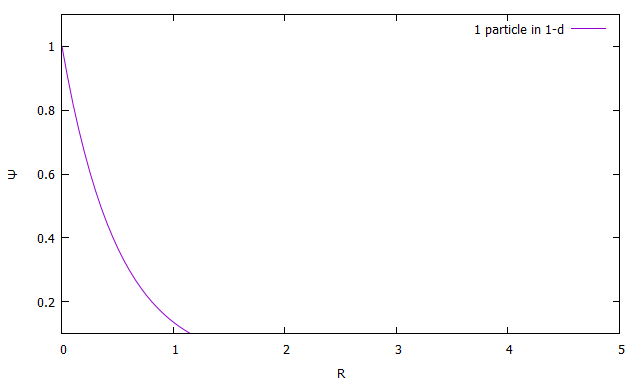
\includegraphics[width=\textwidth]{Psi.png}
	\caption{The one-dimensional wave function of one electron \label{oneparticle}}
\end{figure}

Our program reads in the desired number of grid points, $n$, and the desired integration limits $a$ and $b$. After that, it starts an algorithm to calculate the weights $w_i$ and zeros $x_i$ of a Legendre polynomial of the desired degree $n$ and to save them in arrays. This algorithm is taken from the source-code \glqq exampleprogram.cpp\grqq from the project folder for this course on Github. After calculating the weights and zeros, the algorithm performs a sextuple loop over the arrays and to sum up the weighted values of the function at those points and returns the result:
\begin{lstlisting}
double legendre(int n, double a, double b){
double * x = new double [n];
double * w = new double [n];
gauleg(a, b, x, w, n);
double integral = 0;
for (int i=0; i<n; i++){
for (int j=0; j< n; j++){
for (int k=0; k<n; k++){
for (int l=0; l<n; l++){
for (int y=0; y<n; y++){
for (int z=0; z<n; z++){
integral += (w[i] * w[j] * w[k] * w[l] * w[y]* w[z]
* function_cartesian(x[i], x[j], x[k], x[l], x[y], x[z]));
}}}}}}
return integral;
delete x;
delete w;
\end{lstlisting}
The function \emph{function\_cartesian} simply returns the function value at a given point.

In tab. \ref{results_leg}, you can see the results of this method for some different values of $n$ and some different intervals $[-a,a]$. It is very obvious that these results did not turn to be stable at all. Nevertheless, the computation time was already very high for $n=20$, as we had to perform roughly $n^6$ operations! Remember that the analytical value of the integral is $\frac{5\pi}{256}$.
\begin{table}[h]
	\caption{Results and computation time using Gauss-Legendre\label{results_leg}}
	\centering
	\begin{tabular}{lcccr}
		$n$	&	$a=1$	&	$a=2$	&	$a=5$	&	time $t/\mathrm{s}$	\\\hline
		5	&	0.202983	&	0.354602	&	0.0423687	&	<0.1	\\
		10	&	0.151093	&	0.129834	&	0.0111647	&	0.235	\\
		20	&	0.16142	&	0.177065	&	0.0967888	&	15.896	\\
		25	&	0.163018	&	0.18911	&	0.240135	&	59.496	\\
		30	&	0.163214	&	0.185796	&	0.146371	&	182.404		
	\end{tabular}
\end{table}

To improve the results, we tried calculating the integral with Gauss-Laguerre quadrature. The standard integration limits of Laguerre polynomials are $[0,\inf]$ and the polynomials are suited for functions of the form $x^\alpha\cdot \mathrm{e}^{-x}$. This fits perfectly to our case when we change to spherical coordinates:\\
The integral
\begin{equation}
	\int_{-\infty}^{\infty} d\mathbf{r_1}d\mathbf{r_2}\mathrm{e}^{-4(r_1+r_2)}\frac{1}{|\mathbf{r_1}-\mathbf{r_2}|}
\end{equation}
can now be written as
\begin{equation}
	\int_{-\pi}^{\pi}\left(\int_{-\pi}^{\pi}\left(\int_{0}^{\pi}\left(\int_{0}^{\pi}\left(\int_{0}^{\infty}\left(\int_{0}^{\infty}\left(r_1^2r_2^2\sin(\theta_1)\sin(\theta_2)\mathrm{e}^{-4(r_1+r_2)}\frac{1}{|\mathbf{r_1}-\mathbf{r_2}}\right)dr_1\right)dr_2\right)d\theta_1\right)d\theta_2\right)d\phi_1\right)d\phi_2
\end{equation}
which perfectly fits to the form of Laguerre polynomials if we substitute $r_i'=4r_i$. Note that we have to change the Jacobian accordingly! Now we can solve the integral by applying Gauss-Laguerre quadrature for the two integrals over $r_i'$ and by using Gauss-Legendre for the integrals over the angles.

This program takes the same number of grid points as for Gauss-Legendre. Our algorithm again sets up the weights and zeros for both methods in arrays by using algorithms from the course folder on Github. Then it calculates the weighted function values in a sextuple for-loop, sums them up and returns the integral:
\clearpage
\begin{lstlisting}
double laguerre_legendre(int n){
double * xlag = new double[n+1];
double * wlag = new double[n+1];
double * xphi = new double[n];
double * wphi = new double[n];
double * xtheta = new double[n];
double * wtheta = new double[n];
double a, b;
a=0;
b=2*M_PI;
gauleg(a, b, xphi, wphi, n);
a=0;
b=M_PI;
gauleg(a, b, xtheta, wtheta, n);
//alpha=2 because of r^2 in Jacobian!
gauss_laguerre(xlag, wlag, n, 2.);
double integral=0;
for (int i=1; i<= n; i++){
for (int j=1; j<= n; j++){
for (int k=0; k<n; k++){
for (int l=0; l<n; l++){
for (int y=0; y<n; y++){
for (int z=0; z<n; z++){
//integral+=(laguerre weights)*(legendre weights*function value)*(Jacobian)
//NOTE: Substituted r_1 and r_2 by r_1'=4*r_1 and r_2'=4*r_2!
//Same in "function_spherical"! Changes Jacobian!
integral+=((wlag[i]*wlag[j])*(wphi[k]*wphi[l]*wtheta[y]*wtheta[z]
*function_spherical(xlag[i], xlag[j], xphi[k], xphi[l], xtheta[y], xtheta[z]))
*(sin(xtheta[y])*sin(xtheta[z])))/4096;
}}}}}}
return integral;
}
\end{lstlisting}
Note that in this case the function \emph{function\_spherical} only contains the parts of the function that are not absorbed in the Laguerre weights! Also look at the new Jacobian and the factors we had to add as we made the substitution $r_i'=4r_i$.

In table \ref{results_lag}, you can see the results of the Gauss-Laguerre quadrature. They converge much faster than the results we obtained with 'brute force' Gauss-Legendre and lead to a higher precision. Note that they still need a long computation time!

\begin{table}[h]
	\caption{Results and computation time using Gauss-Laguerre\label{results_lag}}
	\centering
	\begin{tabular}{lcr}
		$n$	&	Integral	&	time $t/\mathrm{s}$	\\\hline
		5	&	0.17345	&	0.017	\\
		10	&	0.186457	&	0.381	\\
		20	&	0.191082	&	26.538	\\
		25	&	0.191741	&	100.167	\\
		30	&	0.192114	&	298.406	
	\end{tabular}
\end{table}

\subsection{Monte-Carlo integration}

We calculated the same integral with Monte-Carlo method. First, we calculated the integral in a brute force way. This means that we calculate the integral using (pseudo) random numbers, which obey uniform distribution functions. The random numbers for each of the six dimensional integral are uniform distributed in a chosen interval (-a to a ). Furthermore, we don't transform the integral, but we calculate it in Cartesian coordinates. We got the values in table \ref{Data from the brute force montecarlo algorithm (part c))}. (We used the interval for a=2 ) In one dimension, the Monte-Carlo method can be described by formula \ref{integralbrute}. 

\begin{align}
I &= \int_{a}^{b} f(x) dx \approx < f(x) > \cdot (b-a) = \frac{1}{n} \sum_{i=1}^{n} f(x_i) \cdot (b-a) = \hat{I} \label{integralbrute}
\end{align}
 
In addition to that, we tried to improve our calculations. First, we transformed the integral into spherical coordinates. In spherical coordinates, we use the variables $\theta$ ( from 0 to $\pi$), $\phi$ (from 0 to 2$\pi$) and r (from 0 to infinity) instead of using Cartesian coordinates $x_{i,k} \ [-\infty$ t $\infty$ ) (i=1,2,3; k=1,2). We also used a distribution function in order to get appropriate values of the random numbers.  Formula \ref{P(x)} to \ref{with distribution} describe the general one dimensional reformulation if you want to use a other particle distribution function. 


\begin{align}
&P(x) = \int_{0}^{x} p(x) dx \label{P(x)}\\
& I =  \int_{a}^{b} \frac{f(x)}{p(x)} \cdot p(x) dx = \cdot \int_{a}^{b} \hat{f}(x) \cdot p(x) dx \approx  \frac{1}{n} \sum_{i=1}^{n} \hat{f}(y_i) \cdot (b-a) = \hat{I} \\
&y_i(x_i) =P^{-1}\left(p(y(x_i))\right)= P^{-1}(x_i)\label{with distribution}
\end{align}
In order to improve the precision of the integral, we used a not uniform distribution function, which can be found in formula \ref{inourcase}ff. 
\begin{align}
P(x)&= \int_{0}^{x} 4 \cdot e^{-4 x} = 1- e^{-4x} \label{inourcase}\\
y_i(x_i)&= -\frac{1}{4} ln(1-x_i)
\end{align}
We transformate the integral to spherical Coordinates and use the distribution function for $r_1$ and $r_2$. Finally, the integral can be calculated through formula \ref{integralinourcase}. The results are in table \ref{Data from the  montecarlo algorithm (part d))}.
\begin{align}
f( r_{1,i}, r_{2,i}, \theta_{1,i}, \theta_{2,i}, \phi_{1,i}, \phi_{2,i}) = \frac{r_{1,i}^2 \cdot r_{2,i}^2 \cdot sin(\theta_{1,i}) sin(\theta_{2,i}) }{\sqrt{r_{1,i}^2+r_{2,i}^2-2 \cdot r_{1,i} r_{2,i}  cos(\theta_{1,i}) cos(\theta_{2,i}) + sin(\theta_{1,i}) sin(\theta_{2,i}) \cdot cos(\phi_{1,i}-\phi_{2,i})}\cdot 4^2}
\end{align}

\begin{align}
\hat{I}= \frac{1}{n} \sum_{i=1}^{n} f( r_{1,i}, r_{2,i}, \theta_{1,i}, \theta_{2,i}, \phi_{1,i}, \phi_{2,i}) \cdot (2 \pi - 0)^2 \cdot (\pi -0)^2  \label{integralinourcase}
\end{align}

\begin{table}[h]
\centering
\caption{Data from the brute force Monte-Carlo algorithm (part c))}
\label{Data from the brute force montecarlo algorithm (part c))}
\begin{tabular}{c|c|c|c}
n & Integral & Standard deviation & Time in s \\
\hline\hline
$10^2$ & 0.06 & 0.04 & 0 \\
$10^3$ & 0.2 & 0.2 & 0.001 \\
$10^4$ & 0.10 & 0.03 & 0.006 \\
$10^5$ & 0.16 & 0.02 & 0.062 \\
$10^6$ & 0.178 & 0.008 & 0.667 \\
$10^7$ & 0.189 & 0.003 & 6.645 \\
$10^8$ & 0.1917 & 0.0009 & 70.881 
\end{tabular}
\end{table}

\begin{table}[h]
\centering
\caption{Data from the Monte-Carlo algorithm with distribution function (in spherical coordinates) (part d))}
\label{Data from the  montecarlo algorithm (part d))}
\begin{tabular}{c|c|c|c}
n & Integral & Standard deviation & Time in s \\
\hline\hline
$10^2$ & 0.22 & 0.08 & 0 \\
$10^3$ & 0.17 & 0.02 & 0.002 \\
$10^4$ & 0.186 & 0.009 & 0.021 \\
$10^5$ & 0.196 & 0.003 & 0.21 \\
$10^6$ & 0.193 & 0.001 & 2.07 \\
$10^7$ & 0.1926 & 0.0003 &  19.49
\end{tabular}
\end{table}

\subsection{Improving our code with parallelization and vectorisation}

In order to use the full computational capability of our machines, we decided to vectorise and parallelize our code. Computations without parallelization use usually only one of the processors of our computer. However, most of the modern computers have more than one processor. Therefore, it makes sense to split up the "work" for one processor and spread it on all from the computer available processors. This is called parallelization. To be able to use parallelization, you have to include a library, a compiler flag and you have to add a few commands to your source code. (An example can be seen in source code below figure \ref{code for parallel} )


\begin{figure}[h]
\caption{code for parallelization}
\label{code for parallel}
\begin{lstlisting}
/* Extract of source code for part c) to explain the application of parallelization.
We also included compiler flags and a library; 
see the source code on Github for further information. 
(link can be found in the end of this report) */
#include <omp.h>
...
int main(){
    int num_threads = omp_get_num_procs(); /*get the number of processors */
    omp_set_num_threads(num_threads); /*set the number of processors */
...
# pragma omp parallel for reduction(+:sum1) reduction(+:sum2) 
  private (i, x1, x2, y1, y2, z1, z2, fofx) /*this belongs to the line above. 
  definition of private variables. 
  This variables are not generally available
  The sums (sum1,sum2) are "shared" variables */
    for(i=0;i<n;i++){
        x1=ran0(&k)*factor-0.5*factor;
        x2=ran0(&k)*factor-0.5*factor;
        y1=ran0(&k)*factor-0.5*factor;
        y2=ran0(&k)*factor-0.5*factor;
        z1=ran0(&k)*factor-0.5*factor;
        z2=ran0(&k)*factor-0.5*factor;
        fofx=exp(-4*(sqrt(x1*x1+y1*y1+z1*z1)+sqrt(x2*x2+y2*y2+z2*z2)));
        fofx=fofx/sqrt((x1-x2)*(x1-x2)+(y1-y2)*(y1-y2)+(z1-z2)*(z1-z2));
        sum1+=fofx;
        sum2+=fofx*fofx;
    }
...
}
\end{lstlisting}
\end{figure}

With parallelization we could speed up our program. For the brute force Monte Carlo integration, we got the results in table \ref{Data from the brute force montecarlo algorithm (part c)) with vec and para}. With parallelization the program is about 3.8 times faster (for instance for n=$10^8$: without parallel 70.881 seconds - with parallel 18.79 s )
In part d, the optimization (parallel., vector.) leads to a decrease of Compilation time up to a factor of 13.5 ! The results of part d with parallelization can be found in table \ref{Data from the  montecarlo algorithm with vectorization and parallelization (part d))}. As a conclusion, we can say that optimizations of the code in terms of using parallelization (and vectorisation; however the contribute of vectorisation wasn't that big in our case) can save a lot of compilation time and is quite easy to use. For big computations, a factor of up to 13.5 can save days. (This could also mean to save much money in case you run your program on a super computer!)

\begin{table}[h]
\centering
\caption{Data from the brute force Monte-Carlo algorithm with parallelization and vectorization (part c))}
\label{Data from the brute force montecarlo algorithm (part c)) with vec and para}
\begin{tabular}{c|c|c|c}
n & Integral & Standard deviation & Time in s \\
\hline\hline
$10^3$ & 0.14 & 0.08 & 0 \\
$10^4$ & 0.22 & 0.05 & 0.004 \\
$10^5$ & 0.18 & 0.01 & 0.02 \\
$10^6$ & 0.187 & 0.009 & 0.181 \\
$10^7$ & 0.196 & 0.003 & 1.859 \\
$10^8$ & 0.192 & 0.001 & 18.79
\end{tabular}
\end{table}

\begin{table}[h]
\centering
\caption{Data from the Monte-Carlo algorithm with distribution function, parallization and vectorization used (integral in spherical coordinates) (part d))}
\label{Data from the  montecarlo algorithm with vectorization and parallelization (part d))}
\begin{tabular}{c|c|c|c}
n & Integral & Standard deviation & Time in s \\
\hline\hline
$10^2$ & 0.20 & 0.06 & 0\\
$10^3$ & 0.19 & 0.03 & 0\\
$10^4$ & 0.189 & 0.010 & 0 \\
$10^5$ & 0.198 & 0.004 & 0.016 \\
$10^6$ & 0.192 & 0.001 & 0.153 \\
$10^7$ & 0.1919 & 0.0003 & 1.488 \\
$10^8$ & 0.1917 & 0.0001 & 14.935 
\end{tabular}
\end{table}

\newpage

\section{Comparison and discussion of the results}

All in all it can be said that Gauss-Legendre quadrature is not suitable at all for integrals of the type we dealt with, having infinite integration limits. The results we observed converge very slowly, respectively no convergence could be observed at all. However the Gauss-Laguerre quadrature fitted much better for the limits of our integral in spherical coordinates. Using this method we observed fast converging results. One drawback of all Gaussian quadrature methods is that the computation time increases by $n^d$, with d being the dimensions we integrate in total and n being the number of integration points. As a consequence Gaussian quadrature is the method of choice only in low dimensional integration problems.
Monte Carlo integration is the method of choice when we want to calculate integrals in higher dimensions. The computation time for Monte Carlo integration is proportional to the number of integration points multiplied with the dimension of the integral. One advantage of the Monte Carlo integration is that it behaves like a real measurement with respect to statistics. Thus, properties like the standard deviation and variance (or even covariance) can be taken to describe the accuracy of the simulation. This is not the case for many other integration methods like Gaussian quadrature. If we compare the results of the Monte Carlo integration (MC) with and without importance sampling, we see that for a standard deviation of 0.003 we get a computation time of 6.645 for the brute force MC and 0.21 for the MC with importance sampling. The importance sampling decreases computation time for the same standard deviation a lot. For MC we used $6 \cdot 10^{8}$ as an upper limit for the amount of random numbers. This is less than the period of the random number generator we used ($10^{9}$). The standard deviation decreases with increasing numbers of integration points in both cases (brute force/importance sampling). This project has shown the usefulness of Monte Carlo methods- especially with importance sampling- for numerical integration of higher dimensional Integrals. 

% WE LOVE MONTE CARLO !!


\section{Source code}

All the source code to this project can be found at Github:

\url{https://github.com/vincentn1/Project-3/}

\end{document}